%%%%%%%%%%%%%%%%%%%%%%%%%%%%%%%%%%%%%%%%%%%%%%%%%%%%%%%%%%%%%%%%%%%%%%%%%%%%%%%%
%2345678901234567890123456789012345678901234567890123456789012345678901234567890
%        1         2         3         4         5         6         7         8

\documentclass[letterpaper, 10 pt, conference]{ieeeconf}  % Comment this line out
                                                          % if you need a4paper
%\documentclass[a4paper, 10pt, conference]{ieeeconf}      % Use this line for a4
                                                          % paper

\IEEEoverridecommandlockouts                              % This command is only
                                                          % needed if you want to
                                                          % use the \thanks command
\overrideIEEEmargins
% See the \addtolength command later in the file to balance the column lengths
% on the last page of the document

\pdfminorversion=4

% The following packages can be found on http:\\www.ctan.org
%\usepackage{graphics} % for pdf, bitmapped graphics files
%\usepackage{epsfig} % for postscript graphics files
%\usepackage{mathptmx} % assumes new font selection scheme installed
%\usepackage{times} % assumes new font selection scheme installed
%\usepackage{amsmath} % assumes amsmath package installed
%\usepackage{amssymb}  % assumes amsmath package installed
\usepackage{amsmath}    			% ams packages for mathematics environment    
\usepackage{amssymb}
\usepackage{amsfonts}
%\usepackage{amsthm}

\usepackage{graphicx}  				% Versatile graphics manipulation options

\usepackage[croatian]{babel}  % Croatian typographical rules and hyphenation patterns 
\usepackage[utf8]{inputenc}  	% Encoding of Croatian characters
\usepackage[T1]{fontenc}
\usepackage{ae,aecompl}     	% Type 1 fonts, similar to Computer Modern

\usepackage{microtype}				% Improves spacing

\usepackage{subfig}
\usepackage{subcaption}

\usepackage{tabularx}
\usepackage{booktabs}
%\newcolumntype{C}{>{\centering\arraybackslash}X} % centered version of "X" type
\setlength{\extrarowheight}{1pt}
\usepackage{enumerate}				% Additional options for listing of items in enumerate environment
\usepackage{todonotes}				% Adding todo items
\usepackage{dirtree}					% Simple display of directory tree
\usepackage{hyperref}					% Managing cross-referencing


\usepackage{lmodern}
\usepackage{nccmath}
\usepackage[keeplastbox]{flushend}
\usepackage{scalerel,stackengine}
\stackMath
\newcommand\reallywidehat[1]{%
	\savestack{\tmpbox}{\stretchto{%
			\scaleto{%
				\scalerel*[\widthof{\ensuremath{#1}}]{\kern.1pt\mathchar"0362\kern.1pt}%
				{\rule{0ex}{\textheight}}%WIDTH-LIMITED CIRCUMFLEX
			}{\textheight}% 
		}{2.4ex}}%
	\stackon[-6.9pt]{#1}{\tmpbox}%
}
\parskip 1ex

%Additional packages
\usepackage{mathptmx}
\usepackage{graphicx, subcaption}
\usepackage{array}
\usepackage{booktabs}
\usepackage[ruled, vlined, linesnumbered]{algorithm2e}
\usepackage{cleveref}
\renewcommand{\algorithmautorefname}{Algorithm}
\SetKwInput{KwPersistent}{Persistent variables}
\SetKwInput{KwLocal}{Local variable initializations}
\SetArgSty{textnormal}
\makeatletter
\newcommand{\nosemic}{\renewcommand{\@endalgocfline}{\relax}}% Drop semi-colon ;
\newcommand{\dosemic}{\renewcommand{\@endalgocfline}{\algocf@endline}}% Reinstate semi-colon ;
\newcommand{\pushline}{\Indp}% Indent
\newcommand{\popline}{\Indm\dosemic}% Undent
%\let\oldnl\nl% Store \nl in \oldnl
%\newcommand{\nonl}{\renewcommand{\nl}{\let\nl\oldnl}}% Remove line number for one line
%\newcounter{algoline}
%\newcommand\Numberline{\refstepcounter{algoline}\nlset{\thealgoline}}
%\AtBeginEnvironment{algorithm}{\setcounter{algoline}{0}}
\makeatother

\makeatletter
\newcommand{\removelatexerror}{\let\@latex@error\@gobble}
\makeatother


%calligraphy packages
\usepackage{calrsfs}
\DeclareMathAlphabet{\pazocal}{OMS}{zplm}{m}{n}
\newcommand{\Ca}{\pazocal{C}}
\newcommand{\Oa}{\pazocal{O}}
\newcommand{\Va}{\pazocal{V}}
\newcommand{\Ua}{\pazocal{U}}
\newcommand{\Aa}{\pazocal{A}}
\newcommand{\Ta}{\pazocal{T}}
\newcommand{\La}{\pazocal{L}}

\newcommand{\Ja}{\pazocal{J}}

\graphicspath{{./figures/}}
\usepackage{float}

\title{\LARGE \bf
Decentralized Strategy for Cooperative Multi-Robot Exploration and Mapping
}
\author{Ana Batinovi\'{c}, Juraj Or\v{s}uli\'{c}, Tamara Petrovi\'{c}, Stjepan Bogdan
	\thanks{Authors are with the University of Zagreb, Faculty of Electrical Engineering  and Computing, LARICS Laboratory for Robotics and Intelligent Control Systems, Unska 3, 10000 Zagreb, Croatia
        {\tt\small (ana.batinovic, juraj.orsulic, tamara.petrovic, stjepan.bogdan) at fer.hr}}}

\makeatletter
\newcommand{\removelatexerror}{\let\@latex@error\@gobble}
\newcommand{\mb}[1]{\boldsymbol{#1}}
\newcommand{\norm}[1]{\left\lVert#1\right\rVert}

\makeatother

\begin{document}
\maketitle

\thispagestyle{empty}
\pagestyle{empty}


%%%%%%%%%%%%%%%%%%%%%%%%%%%%%%%%%%%%%%%%%%%%%%%%%%%%%%%%%%%%%%%%%%%%%%%%%%%%%%%%
\begin{abstract}

This work presents a novel approach to autonomous decentralized multi-robot frontier exploration and mapping of an unknown area.  The mobile robot team simultaneously explores the environment, discovers frontier points (points on the border between the explored and unexplored space), and communicates by fully connected graph and event-based communication in order to become dispersed throughout the environment. During the exploration, the amount of information exchanged between the robots is limited to data about the robot positions and their current target points. The main goal is to allocate the mobile robots to target frontier points in the environment in a way which minimises the overall exploration time. Moreover, mobile robots creates common map of the environment. The proposed strategy has been implemented in a simulation environment and compared with a coordinated exploration strategy. The simulation results demonstrate the effectiveness of the proposed decentralized multi-robot strategy.

\end{abstract}
\section{INTRODUCTION}
Analysis and synthesis of decentralised multi-robot systems belong to core robotics problems that have drawn significant attention in last few decades. The coordination of a mobile robot team during the exploration of an unknown area is a common problem encountered in many applications, such as search and rescue \cite{Murphy2004}, cleaning \cite{Endres}, \cite{Pinheiro2015}, warehousing \cite{Wurman2008}, or planetary exploration \cite{Mataric2001}, to name a few. Due to the fact that autonomous multi-robot systems are entering society domain and as such will interact with people on daily basis, development of efficient coordination algorithms becomes inevitable.

 Like in the human world, robots can be more effective when they work together. Moreover, a robot team can accomplish a predefined task much quicker than a single robot can \cite{Dias2000}. Another advantage of mobile robot teams arises from the possibility of merging overlapping sensor information, which in turn can help to compensate for sensor uncertainty \cite{Wurm2008}.
If is done properly, multi-robot coordination can lead to i) task accomplishment in the shortest possible time, ii) increased robustness, iii) higher map quality (in case of exploration task), and finally iv) the completion of tasks impossible for a single robot to perform \cite{Dias2006}.

We consider the problem of an autonomous multi-robot exploration with decentralised coordination strategy based on the market model. The laser scan and odometry sensor measurements of the mobile robot represent input data for a Simultaneous Localisation and Mapping (SLAM) module. In this work, for map building we use a submap-based graph SLAM method -- Google Cartographer \cite{Hess2016} -- which, however, in the simulation uses the ground truth mobile robot poses (\textit {perfect localisation}) from the Stage simulator \cite{stageweb} in order to eliminate the SLAM algorithm uncertainty. The module also implements frontier detection according to \cite{Orsulic2019}. A result of frontier detection are the points on the border of the explored and unexplored space in the environment - \textit{frontier points} shown in the Fig. \ref{fig:environment}. The result of frontier detection is a dense set of frontier points, thus we use a filter to get a more manageable number of the frontier points \cite{Umari2017}. The decentralised strategy based on the market model module acquires the frontier points from the filter module and assigns mobile robots to target points. Afterwards, the algorithm for path planning and following navigates the mobile robot toward the target point (Fig. \ref{fig:exploration-strategy}). 

\begin{figure}{}
    \centering
	\fbox{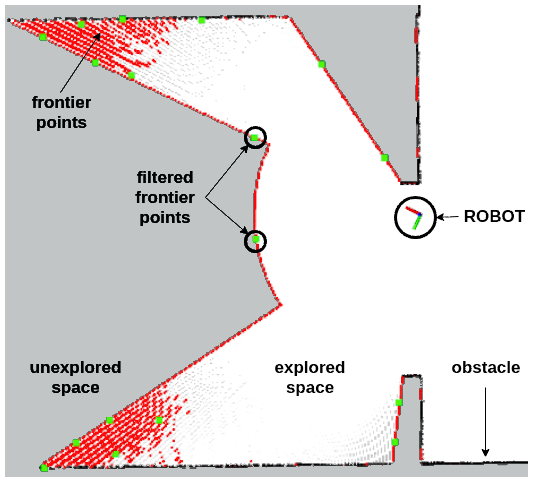
\includegraphics[width=0.85\columnwidth]{./Pictures/frontier_rviz_vol3.png}}
	\caption {The description of the environment. A 2D map is represented with an occupancy grid that divides the map into cells: the white cells describe explored and grey cells unexplored space, while the black cells define obstacles. The frontier detector publishes frontier points (red) and the filter module publishes filtered frontier points (green).}
	\label{fig:environment}
\end{figure}

\begin{figure}
    \centering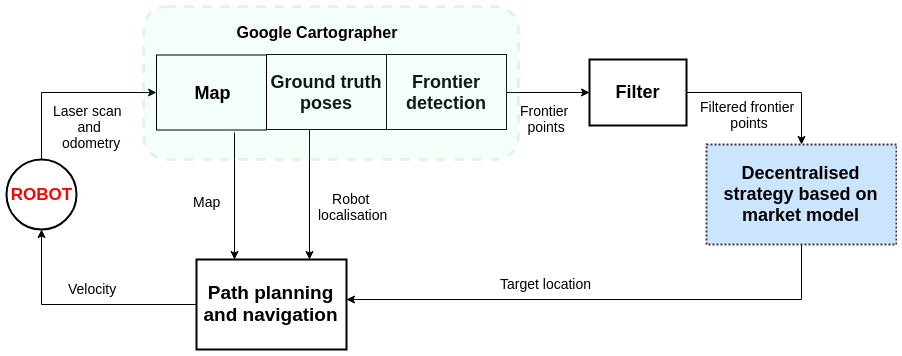
\includegraphics[width=1.0\columnwidth]{./Pictures/diagram_exploration2.png}
	\caption{Overall schematic diagram of the decentralised exploration algorithm in the simulator.}
   \label{fig:exploration-strategy}
\end{figure}

Since the main goal is to achieve faster exploration and better coordination among the mobile robots, our decentralised market-based strategy ensures that the mobile robots become dispersed throughout the environment. Moreover, the mobile robots are dispersed in the environment to accomplish the mission as fast as possible. It is assumed that communication among the mobile robots is modelled by a fully connected graph.

The rest of the paper is organised as follows. The related work is presented in the next section. In Section III the exploration strategy based on market model is described. Simulation results are presented in Section IV, and in the final section a conclusion is given.
\section{EXPLORATION AND MAPPING OVERVIEW}
%\section{EXPLORATION STRATEGY DESCRIPTION}
%Change the title--Method overview
The laser scan and odometry sensor measurements of the mobile robot represent input data for a Simultaneous Localisation and Mapping (SLAM) module. In this work, for map building we use a submap-based graph SLAM method -- Google Cartographer \cite{Hess2016} -- which, however, in the simulation uses the ground truth mobile robot poses (\textit {perfect localisation}) from the Stage simulator \cite{stageweb} in order to eliminate the SLAM algorithm uncertainty. The module also implements frontier detection according to \cite{Orsulic2019}. This method has achieved impressive results in terms of wall-time per frontier update, what greatly speeds up our exploration and mapping process. 

Google Cartographer SLAM extended with frontier detection and filter module are centralized part of the exploration and mapping process (Fig. \ref{fig:exploration-strategy}). Centralized part generates filtered frontier points, inputs to $n$ equal decentralized strategies modules for $n$ mobile robots. During the exploration and mapping $n$ mobile robots communicate, exchange minimum information about frontier points in order to decide where to navigate and create common map of the unknown environment. Focus and scope of the paper is decentralization of the decision making process, using centralized SLAM algorithm and centralized filtered frontier point generator. Further, the algorithm for path planning and following navigates the mobile robot toward the target point. The process is over when the area is explored.  

\begin{figure}[t!]
    \centering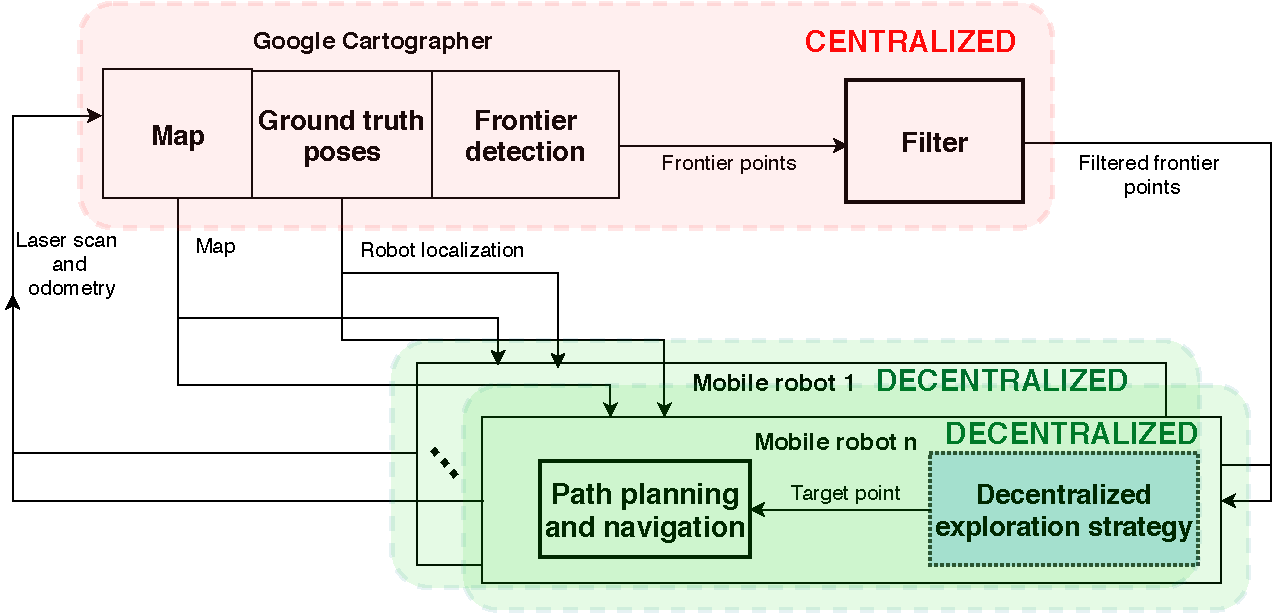
\includegraphics[width=1.0\columnwidth]{./Pictures/diagram_exploration.pdf}
	\caption{Overall schematic diagram of the decentralized exploration and mapping process for $n$ mobile robots in the simulator. Google Cartographer and filter module (highlighted red) generate filtered frontier points that are centralized part of exploration and mapping process. Exploration strategy and path planning and navigation module (highlighted green) are decentralized parts that generate $n$ outputs and create common map.}
   \label{fig:exploration-strategy}
\end{figure}

Our multi-robot exploration and mapping process combine SLAM (Google Cartographer), a frontier detection algorithm, filter module and a decision making strategy. Each component can be easily changed or extended, without affecting an exploration and mapping process. For instance, the decentralized strategy can be replaced without affecting the frontier points detection. Similarly different types of frontier points detectors could be tested without affecting the behaviour of the decision making strategy. The same logic is valid for SLAM method and filter module. This makes our exploration and mapping process more flexible and modular. 

\subsection{SLAM} 
Most literature uses the ROS 'gmapping' package for generating the
map and localizing mobile robots \cite{Keidar2012}, \cite{Umari2017}. The 'gmapping' package implements a SLAM algorithm that uses a Rao-Blackwellized particle filter \cite{Grisetti2007}. 
On the other side, we use Google Cartographer SLAM algorithm \cite{Hess2016}, an open source available in \cite{cartographer}, which in our case generates ground truth map. Cartographer is an open-source 2D and 3D graph SLAM based on occupancy grid submaps. 
An extension to the Cartographer is a new fast frontier detection method developed in \cite{Orsulic2019}. 

\subsection{Frontier Detection}
A popular frontier-based exploration approach is introduced by Yamauchi \cite{Yamauchi1998}, where the robots explore an unknown environment and build a common map. Moreover, each robot heads to the center of mass of the closest frontier and frontier detection is performed only when the robot reaches its target. 
The frontier edges detection can be achieved using RRT (Rapidly Exploring Random Tree) algorithm by Umari and Mukhopadhyay \cite{Umari2017}. The RRT algorithm is biased towards unexplored regions and provides a general approach which can be extended to higher dimensional spaces. However, RRT algorithm proved not to be fast enough in instances when larger parts of the environments were explored, so we opted to use a dense frontier detection method \cite{Orsulic2019}. Orsulic has achieved great results in terms of wall-time per frontier update. Furthermore, this paper is the first usage of the dense frontier detection method in multi-robot exploration and mapping. 

\subsection{Filter Module}

The filter module receives the frontier points from frontier detector  and first clusters the points and stores only the centre of each cluster. The clustering process reduce the number of frontier points from frontier detection module, which are extremely close to each other. If such amount of points are sent to the decentralized exploration strategy module, there would be unnecessary consumption of computational resources, without additional information about the frontier. We use Hierarchical Agglomerative Clustering \cite{clutering} because it does not require predefined number of clusters. We only need to set distance threshold parameter, above which clusters will not be merged. Even though it has a time complexity of ${\displaystyle {\mathcal {O}}(n^{3})}$, it is suitable for our case because of the size of frontier points. Moreover, it is easy to implement. 

\subsection{Why Decentralized?}

Algorithms for assigning robots to target points can be grouped into centralized and decentralized algorithms. Centralized task assignment for a multi-robot system may be less practical due to communication limits \cite{Dias2000}, robustness issues \cite{Dias2006}, or time required for algorithm execution and scalability \cite{Julia2012}. In the centralized approach, each mobile robot receives tasks assigned from a single central \emph{leader} using a centralized planning algorithm. During communication between the central leader and the mobile robots, information about the mobile robot poses is shared in order to perform real time mobile robot task allocation. The central leader may be a computer or a robot. An advantage of centralized approach is that the optimal plans can be found \cite{Yan2011}. Nevertheless, this mechanism is ineffectual for large mobile robot teams.

In contrast to centralized approaches, in a decentralized approach, the mobile robots are completely autonomous in the exploration process. Each mobile robot has its own local knowledge of the world and can decide its future actions by taking into account its current context and task, its own capacities and the capacities of the other mobile robots, through a negotiation process \cite{Yan2013}. Moreover, it usually has better reliability, flexibility, adaptability and robustness \cite{Zlot2002}. There is no central planner in the decentralized multi-robot exploration problem, so mobile robots need to communicate and cooperate effectively to explore and map an unknown environment as soon as possible. 
In order to have more robust and flexible system we propose a strategy in which mobile robots are able to decide toward which target point to navigate, with the assumption that the mobile robots have knowledge of all target points, while we assume that only a single mobile robot can be assigned to a specific target point.  

In this paper we determine the target points for each mobile robot in the team using an objective function which is a combination of frontier point cost, utility of reaching the target point and a novel extension - the frontier occupancy function that makes mobile robot be dispersed throughout the environment. 

\section{DECENTRALIZED EXPLORATION STRATEGY} 

At the core of our paper is a decentralized strategy for multi-robot exploration and mapping. The mobile robots exchange information about frontier points under the assumption of a fully connected graph and event based communication. If we define a mission as a process from getting a target point to reaching the same point, then all mobile robots communicate with each other in the moments when the mission for a single mobile robot is over. It means that the rest of mobile robots should send the data even though their missions are not over and they are still navigating to the goal. Event based communication is triggered by mission accomplishments.   

The exploration task is performed by a team of $n$ mobile robots  \(\text{$\mathcal {R}$}\) = $ \{ 1, 2,..., N\}$ where the mobile robots do not have prior knowledge about the environment, i.e., the position of the boundaries and obstacles.  
Every mobile robot $i$ gets the list of frontier points  \(\text{$\mathcal {Y}$}\) = $ \{ 1, 2,..., M\}$ from filter module (Fig. \ref{fig:exploration-strategy}) in the moments when any of the mobile robots reaches the target point (when the mission is over). $M$ is the number of frontier points represented as a tuple ($x$, $y$), corresponding to the position in meter from the map origin. 

We define the frontier point weight $W$ as a function of cost $C$, utility $U$ and frontier occupancy $F$. Cost function $C$: $R_{xy}$ \(\rightarrow \text{$\mathbb{R}^{+}$}\) is a mapping from $R_{xy}$ to a positive real number.  If $i$ is the index of the mobile robot, and $j$ is the index of the frontier point, then $C_{ij}$ describes the cost of $i$th robot to visit the $j$th frontier point. The cost can be a function of time, energy or, like in our case, the estimated distance travelled by mobile robot to reach the target frontier point. The estimated distance is approximated using Euclidean distance between the mobile robot position $\boldsymbol{p_{i}}$ and the frontier point position $\boldsymbol{y_{j}}$:

\begin{equation}\small
    C_{ij}=d(\boldsymbol{p_{i}}, \boldsymbol{y_{j}}) = \sqrt{(p_{ix}-y_{jx})^{2}+(p_{iy}-y_{jy})^{2}}.
    \label{cost}
\end{equation}

The utility function $U_{ij}$: $R_{xy}$ \(\rightarrow \text{$\mathbb{R}^{+}$}\) returns a positive real number, and uses the occupancy grid \(\text{$\mathcal {M}$}\) to find the value for the specific frontier point. The cells of \(\text{$\mathcal {M}$}\) may be marked as explored space, unexplored space or obstacle. The utility function is proportional to the number of the unexplored cells $c$ within a fixed distance from the frontier point $y_{j}$ in the previous defined radius $r$: 

\begin{equation}
    U_{y_{j}} = \lambda_{u}c,
\end{equation}

where $\lambda_{u}$ is a constant determined experimentally. When the function $U_{y_{j}}$ is taken into account, the mobile robot will prefer frontier points that are surrounded by more unexplored space even if they are a little bit further. 
It is assumed that the mobile robot will detect all unexplored cells around the assigned frontier point after reaching it. 

The most important component is the frontier occupancy function $F_{ij}$, the 2-dimensional Gaussian function with the position of the mean in a frontier point and with the standard deviation \boldsymbol{\sigma} = \begin{bmatrix}
           r_{f} \\
           r_{f} 
   \end{bmatrix}.
   
 If the frontier point $y_{j}$, for which the mobile robot $i$ is calculating the weight, is in the range of radius $r_{f}$ from the position of an another mobile robot assigned point (\boldsymbol{y_{a}}); the value of the frontier occupancy function is calculated by Gaussian function, and zero otherwise:

\begin{equation}\label{eq:frontier_funct}
 F_{ij}=
\begin{cases} 
       \lambda_{f} e^{-\Big[\frac{(y_{jx} - y_{ax})^2}{2\sigma_{x}^2} + \frac{(y_{jy} - y_{ay})^2}{2\sigma_{y}^2}\Big]} & \text{if $d(\boldsymbol{y_{j}}, \boldsymbol{y_{a}})< r_{f}$}, \\
      \quad \quad \quad \quad \quad 0 & \text{otherwise}
   \end{cases}
\end{equation}

where $\lambda_{f}$ is an experimentally determined constant. 
The example of the frontier point $y_j$, assigned point $y_a$ and Gaussian function values inside the radius $r_f$ are shown in Fig. \ref{fig:gauss}.
The function $F_{ij}$ is used to prevent assigning the frontier point to the mobile robot B if that point is close to a point that is already assigned to mobile robot A.

\begin{figure}[t!]
	\centering
	\fbox{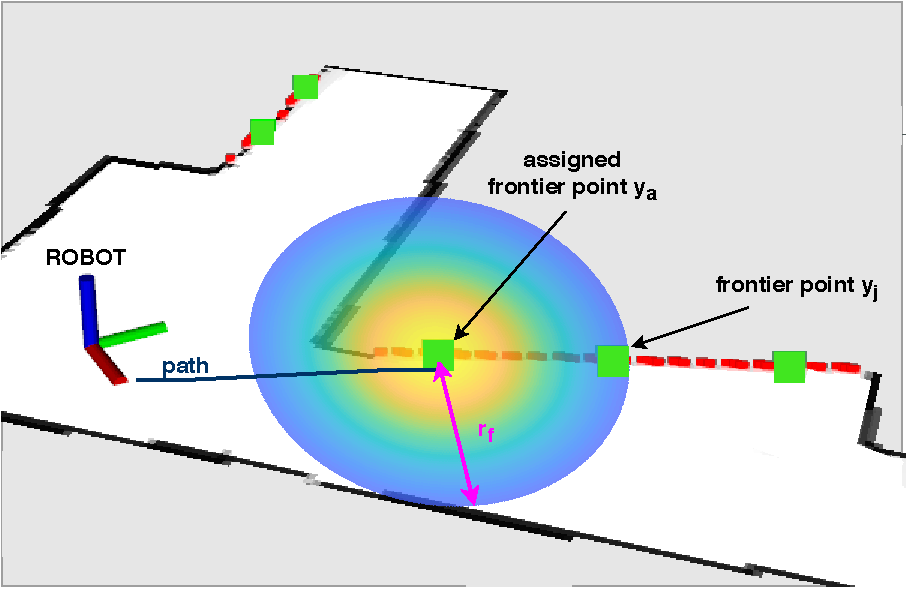
\includegraphics[width=0.95\columnwidth]{./Pictures/gauss.pdf}}
	\caption{A special scenario where the value of the frontier occupancy function $F$ is different from zero. Mobile robot is assigned to frontier point $y_a$, and follows the path to reach it. If another mobile robot calculates weight for the all current frontier points (green points), $F$ for frontier point $y_j$ is different from zero because $y_j$ is inside the radius $r_f$}.
	\label{fig:gauss}
\end{figure}

For each frontier point $y_{j}$, the weight $W_{ij}$ of the $i$-th mobile robot is calculated as: 
\begin{equation}
   {W}_{ij}= {C_{ij}} - {U_{y_{j}}} + {F_{ij}}.
   \label{weight}
\end{equation}

The weight matrix $\boldsymbol{W}$ ($N\times M$) is formed for $N$ mobile robots and $M$ frontier points: 

\begin{equation}
    \boldsymbol{W} = \begin{bmatrix}
    W_{00} & W_{01} & \hdots & W_{0j} & \hdots & W_{0M}\\
    W_{10} & \ddots & & & & \vdots\\
    \vdots & & \ddots & & &  \vdots \\
    W_{i0} & & & \ddots & & \vdots \\
    \vdots & & & & \ddots & \vdots\\
    W_{N0} & \hdots  & \hdots  & \hdots  & \hdots &    W_{NM}
    \end{bmatrix}.
\end{equation}

The mobile robots exchange information about their positions and current target points and make decisions for the future actions based on the exchanged information. The amount of exchanged data is thus reduced, which allows easier and faster communication.
The weight matrix $\boldsymbol{W}$ represents the input into the Hungarian algorithm that attempts to find an optimal assignment solution in polynomial time.

The Hungarian algorithm is described in \cite{Kuhn1955} and tested in \cite{Kulich2015}. Initially, the Hungarian algorithm assumes that the number of frontier points is the same as the number of mobile robots. Due to the fact that there are usually fewer mobile robots than frontier points, virtual mobile robots are added and then skipped during the process of assignment and exploration.

Let the matrix $X$ be the matrix of zeros and ones, where $X[i,j]=1$ iff the mobile robot $i$ is assigned to the frontier point $j$.
Than the optimal task assignment has weight:

\begin{equation}
     {\min_{X}}\ \Big(\sum_{i} \sum_{j} W_{ij}\ X_{ij}\Big),
\end{equation}

anticipating that minimisation of sum will ensure the dispersion of the mobile robots in the environment. 

\begin{algorithm}[t!]
\While{Unexplored}{
\If{Request}{
    Send position and current target point to the other mobile robots\;
    }
\If{Mobile robot $i$ has reached the previous target point}{
    Request positions and current target points from the other mobile robots\;
    \For{Each frontier point $y_{j}$}{
    Calculate the weight matrix $\boldsymbol{W}$\;
    Hungarian algorithm ($\boldsymbol{W}$)\;
    \textbf{return} Mobile robot $i$ is assigned to frontier point\;
    }
}
}
\label{algorithm1}
\caption{Decentralized strategy for mobile robot $i$}
\end{algorithm}


Our decentralized strategy executes during the robot motion and there are steps for each robot to be executed (\textbf{Algorithm 1}). All frontier points are visible to all mobile robots.
When mobile robot $i$ is assigned to frontier point according to line 10 in \textbf{Algorithm 1}, the mobile robot starts to follow the planned path and navigates to the target frontier point. Moreover, at the moment when the mobile robot $i$ reaches the target point (mission is over), a request is sent to the other mobile robots to get their positions and current target points, and to fill in the weight matrix $\boldsymbol{W}$, which is an input to Hungarian algorithm. The described process executes until the whole environment is explored, in other words, until a complete  map of the environment is generated. The Fig. \ref{fig:structure} illustrates the described steps and algorithm lines for a mobile robot team. 

\begin{figure}[h!]
    \centering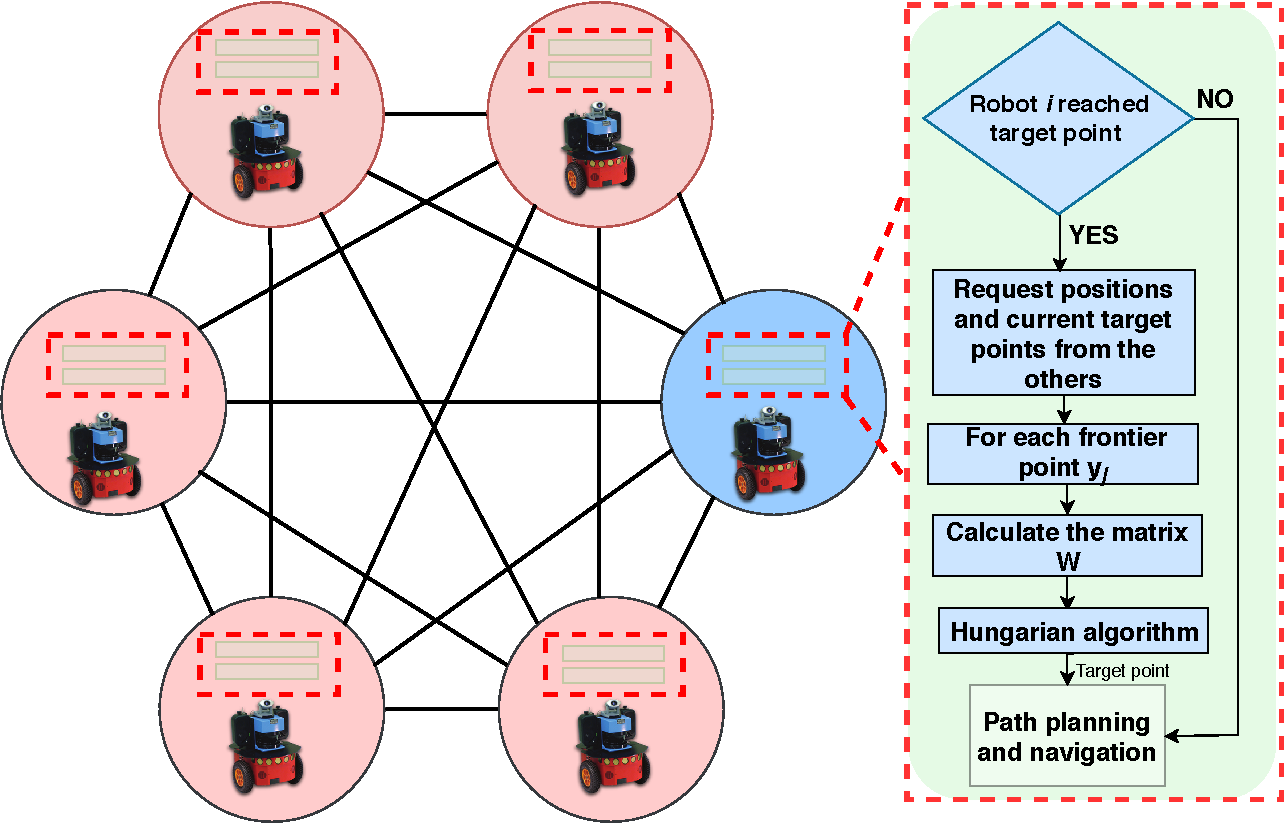
\includegraphics[width=1.0\columnwidth]{./Pictures/struktura_vol1.pdf}
	\caption{An execution of the decentralized part of the Fig. \ref{fig:exploration-strategy}. Every mobile robot explores the environment following the steps from \textbf{Algorithm 1}. The blue robot accomplished the mission and requests weights from the rest team memebers (red ones). The strategy is the same for all mobile robots and starts in the moment when each of them reaches the target point.}
   \label{fig:structure}
\end{figure}


\section{SIMULATION RESULT}

The proposed strategy is implemented and tested using the Robot Operating System (ROS) framework. In order to prove the efficiency of our decentralised strategy, we compared it with the coordinated centralised market model described in \cite{Burgard2005}. Experiments were performed in the two different indoor environments (Fig. \ref{fig:scenarios}) with two, three and five mobile robots. The start pose of the mobile robot was the same for each run. The results are presented as average of 10 runs for each set. The simulation setup is shown in the Table \ref{tab:table1}.


\begin{figure}[t]
    \setcounter{subfigure}{0}
     \begin{center}
        \subfigure[][]{\label{fig:office}
            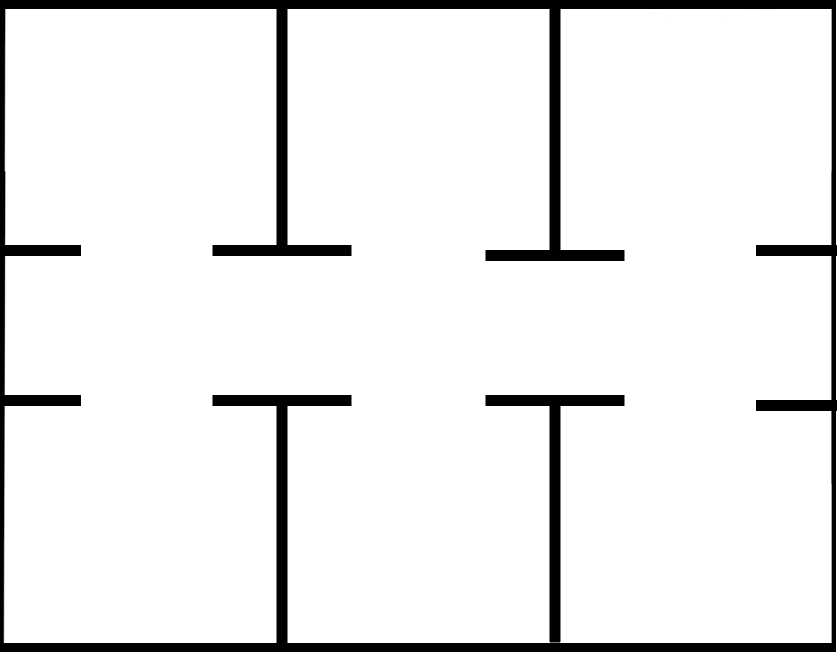
\includegraphics[width=0.47\columnwidth]{office1.png}
        }\hfill
        \subfigure[]{\label{fig:unstructured}
           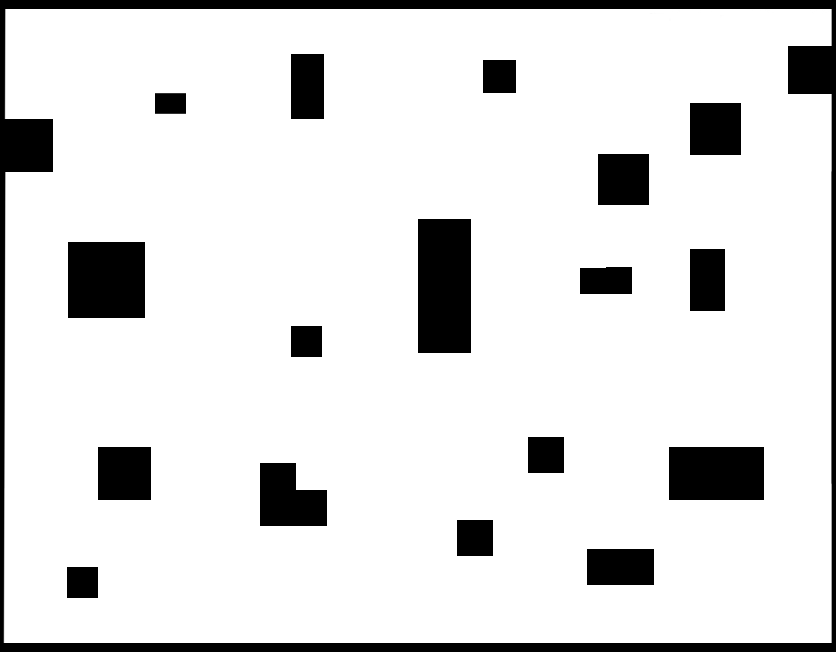
\includegraphics[width=0.47\columnwidth]{unstructured.png}}
    \end{center}
    \caption{%
       Benchmark scenarios. The terrains cover the flat surface 40 x 20 $m^{2}$ with static obstacles. \subref{fig:office} Office-like scenario; \subref{fig:unstructured} Unstructured scenario.
     }%
   \label{fig:scenarios}
\end{figure}




\begin{figure*}[h!]
     \begin{center}
     \setcounter{subfigure}{0}
%
        \subfigure[\hspace{0.1cm} Total exploration time for centralised and decentralised strategy in the office scenario for the different size of the mobile robot team]{%
            \label{fig:tt-office-a}
            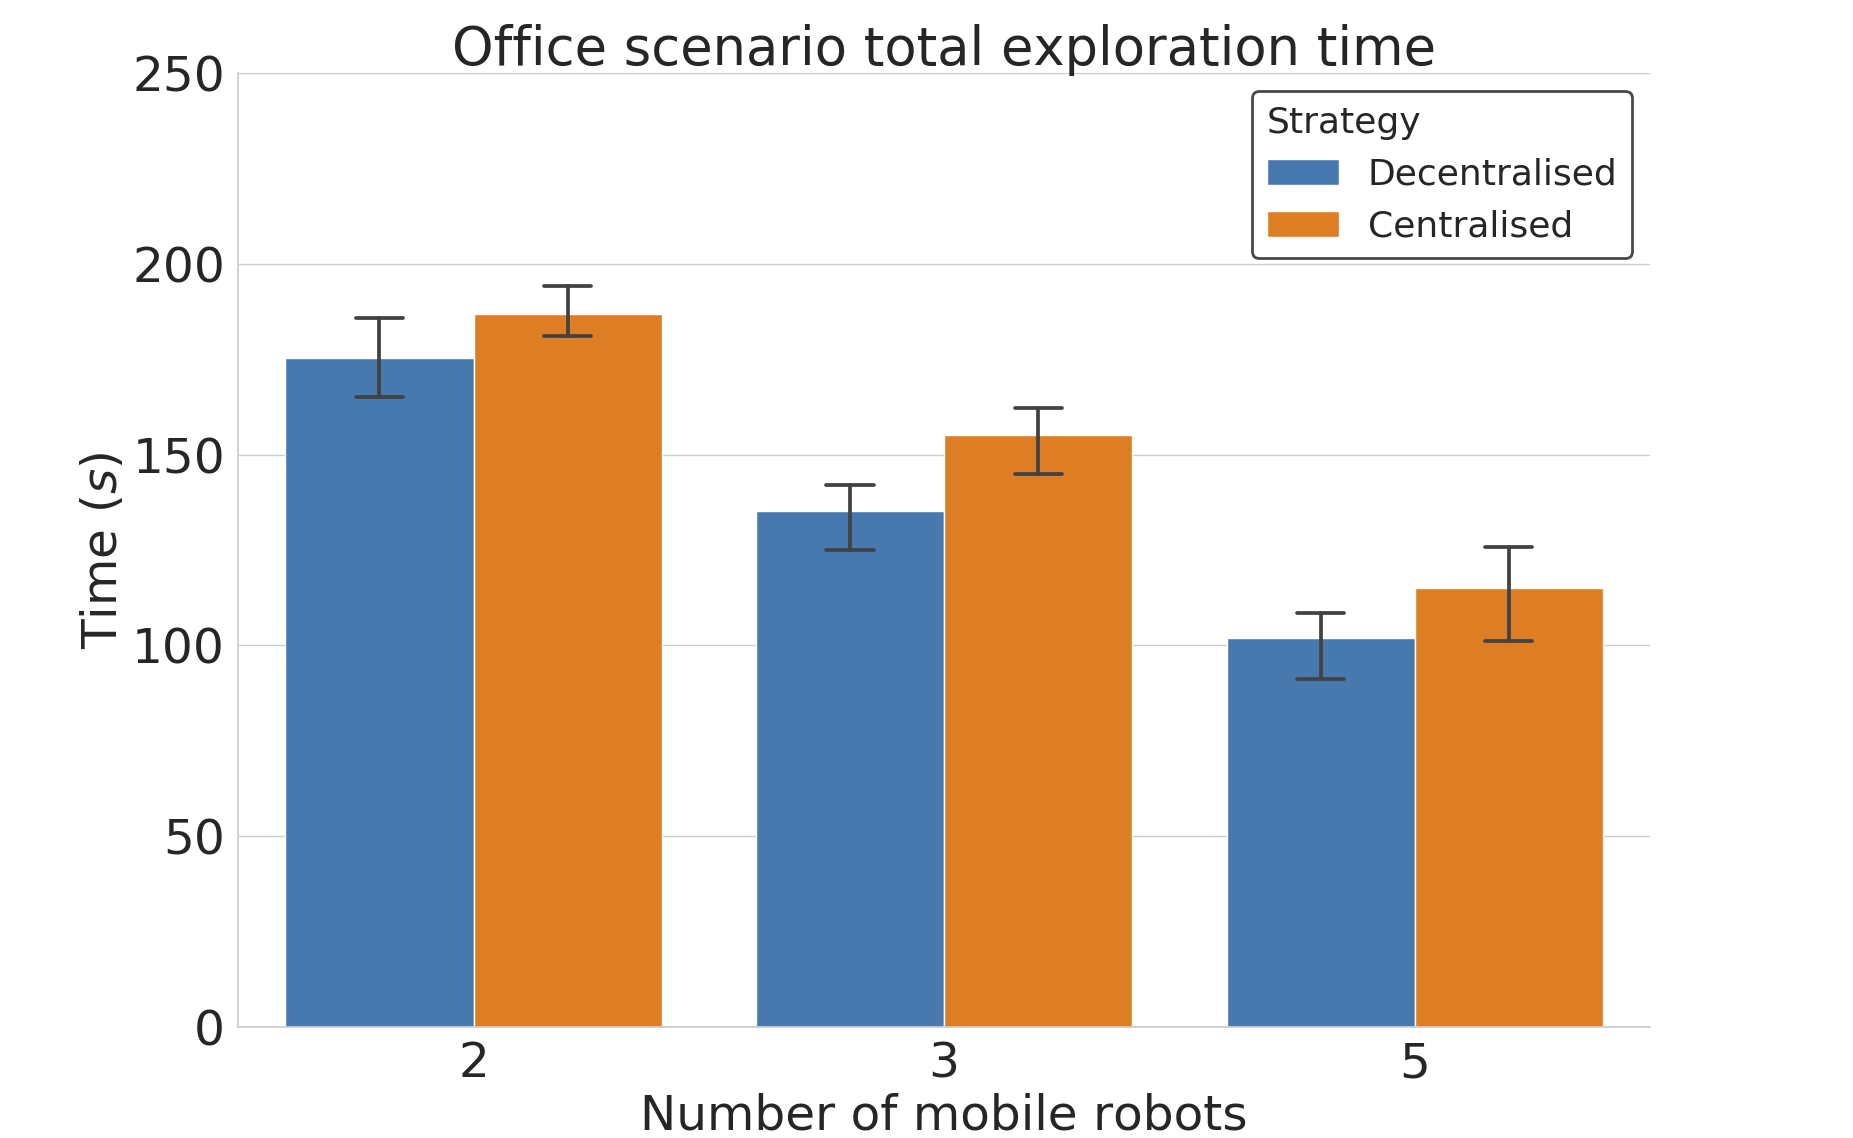
\includegraphics[width=0.46\textwidth]{office_total_e_time.png}
        }\hfill
        \subfigure[\hspace{0.1cm} Total exploration time for centralised and decentralised strategy in the unstructured scenario for the different size of the mobile robot team]{%
           \label{fig:tt-unstructired-b}
           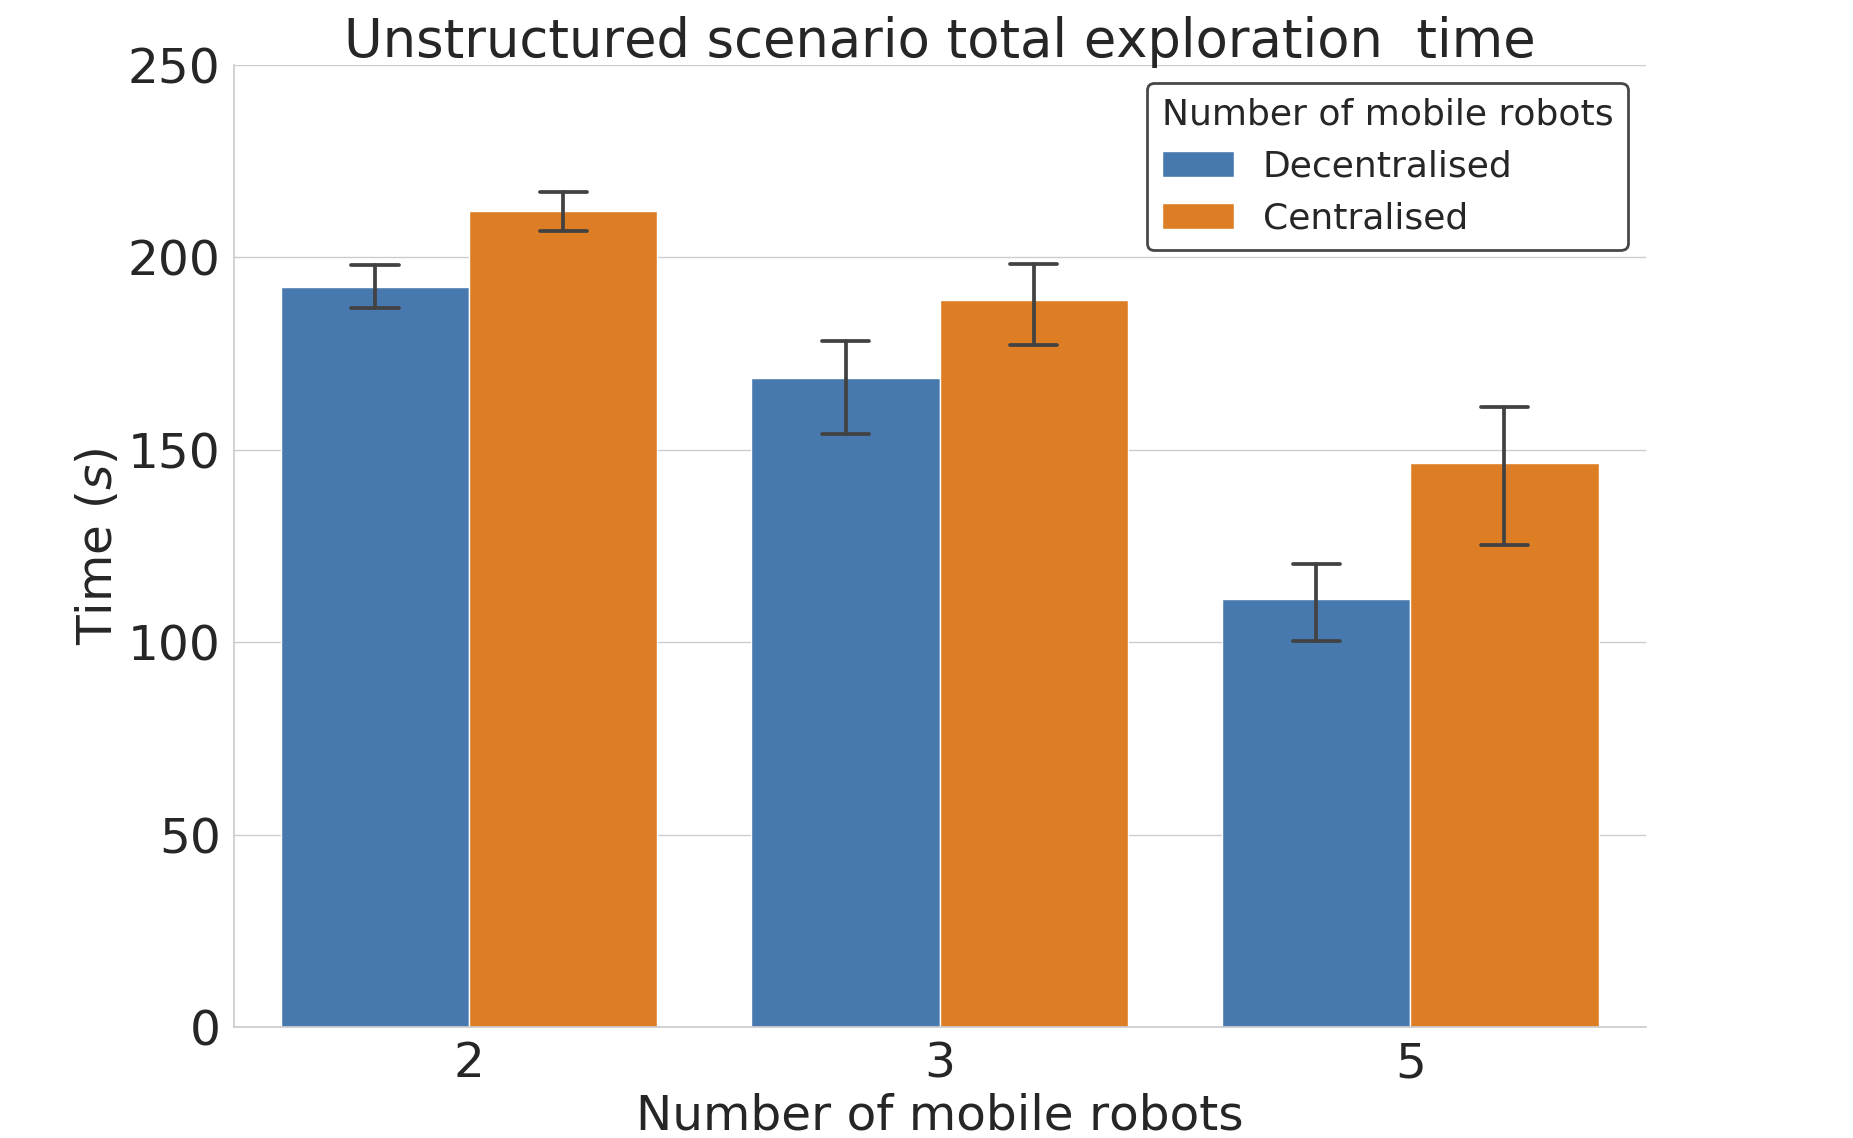
\includegraphics[width=0.46\textwidth]{unstructured_total_e_time.png}
        }\\ %  ------- End of the first row ----------------------%
        \subfigure[\hspace{0.1cm} Average path length per robot for centralised and decentralised strategy in the office scenario for the different size of the mobile robot team]{%
            \label{fig:path-office-c}
            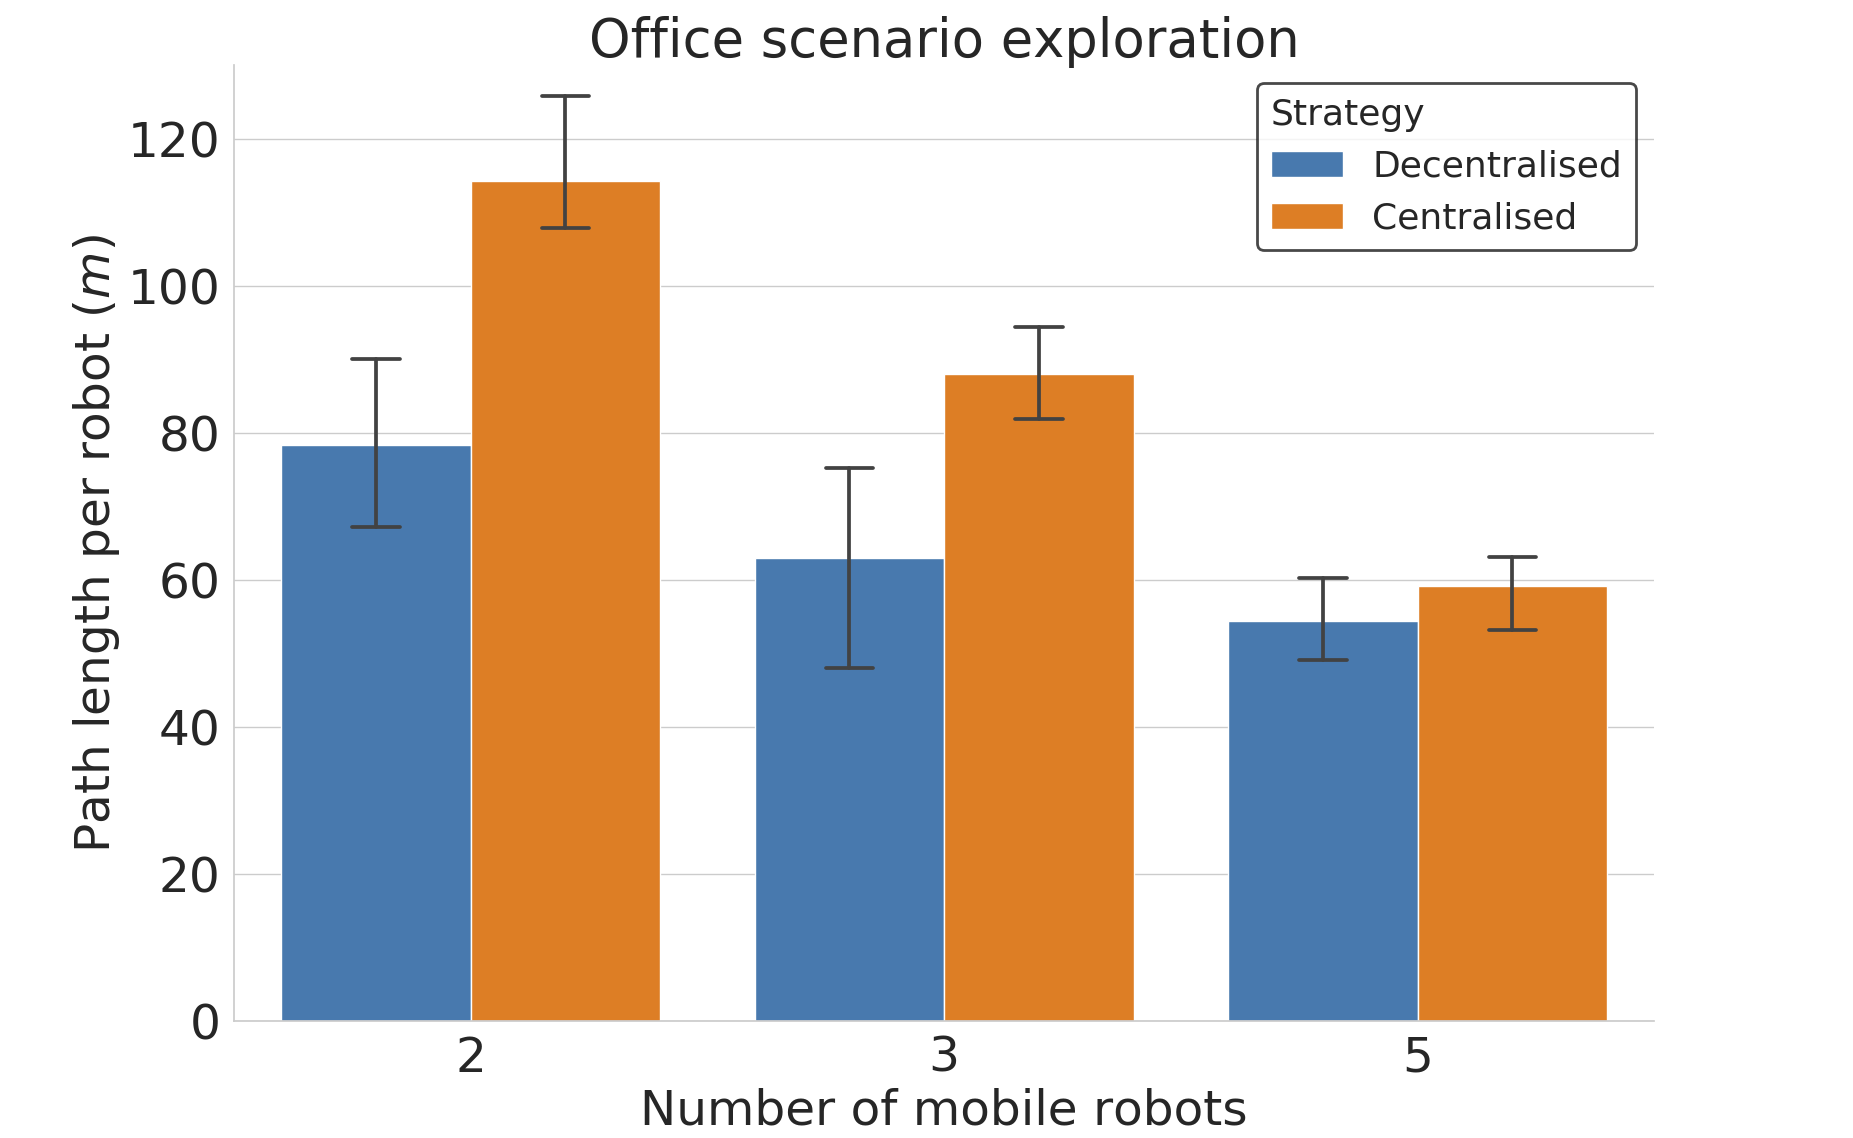
\includegraphics[width=0.46\textwidth]{office_path_length_per_robot.png}
        }\hfill
        \subfigure[\hspace{0.1cm} Average path length per robot for centralised and decentralised strategy in the unstructured scenario for the different size of the mobile robot team]{%
            \label{fig:path-unstructured-d}
            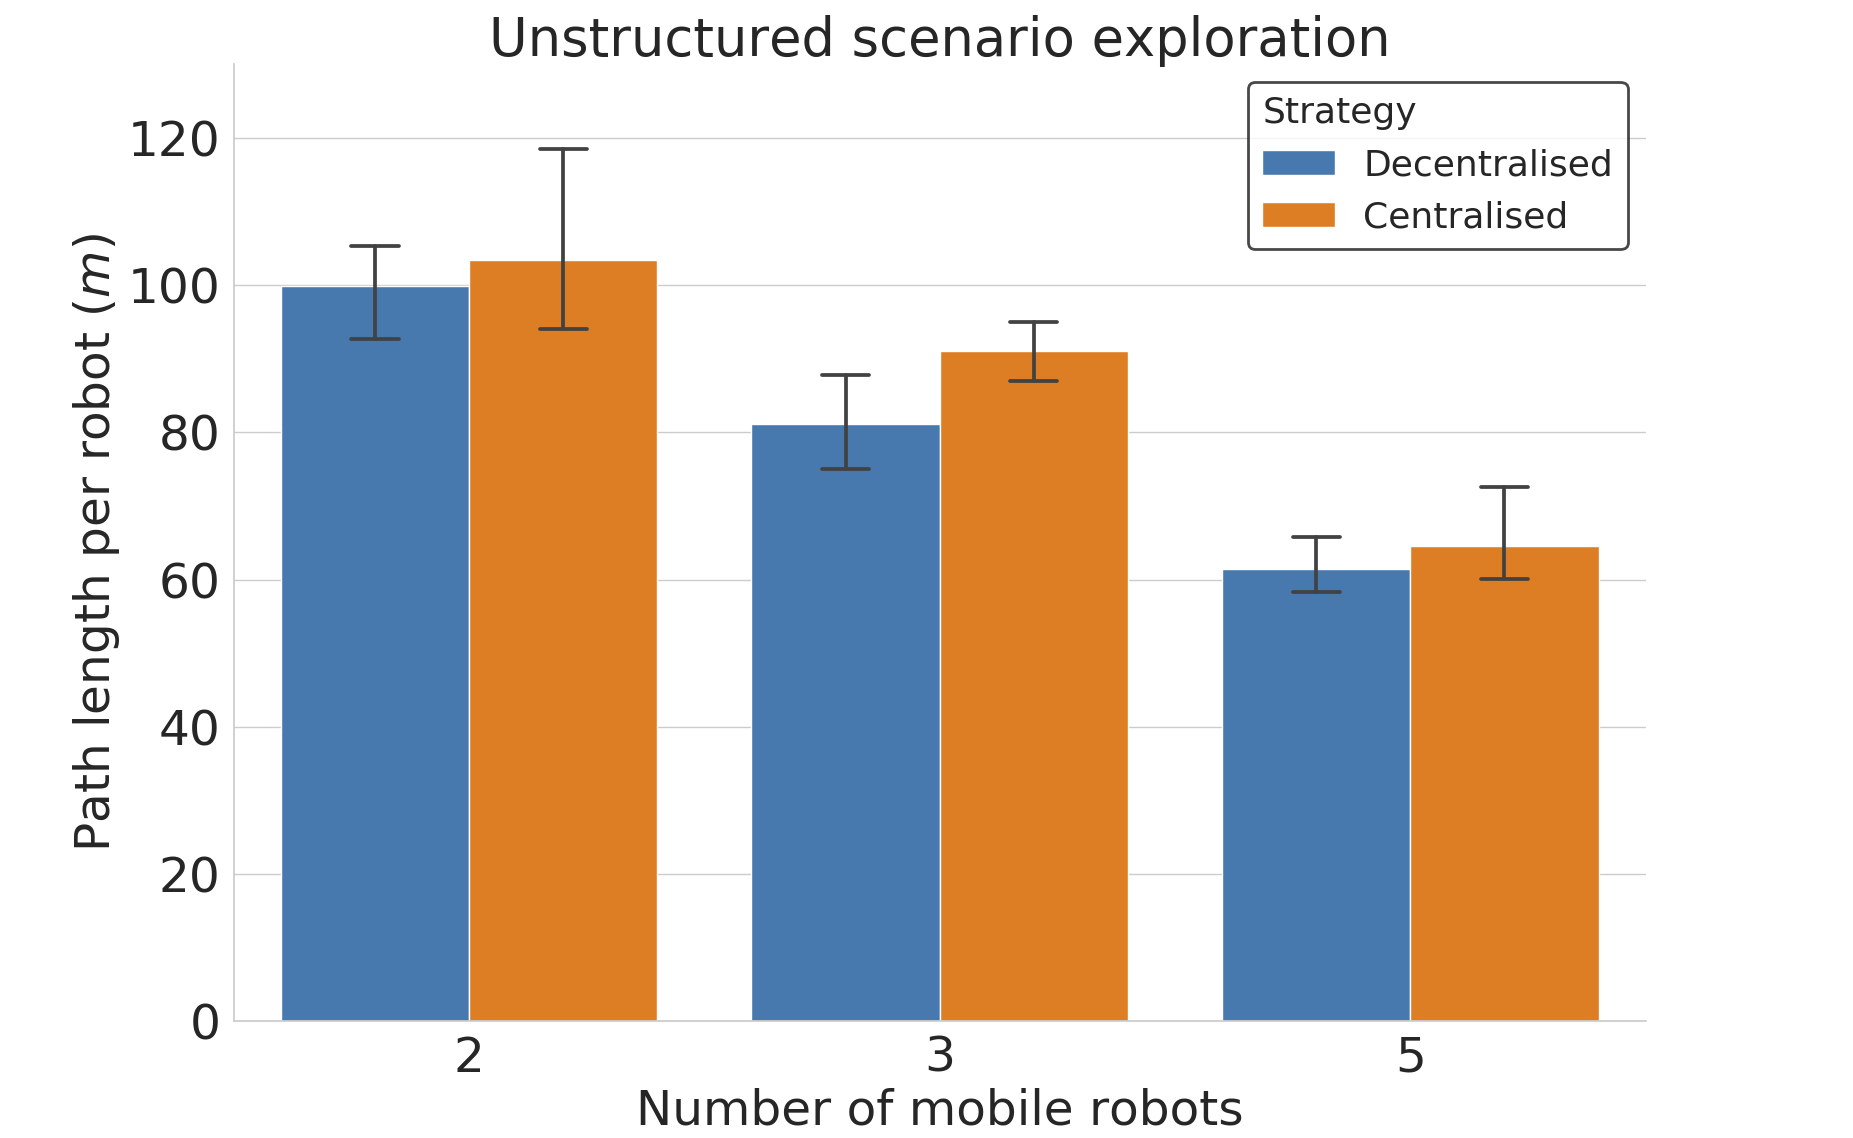
\includegraphics[width=0.46\textwidth]{unstructured_path_lenght_per_robot.png}
        }%
%
    \end{center}
    \caption{%
       The comparison of the centralised and decentralised strategy for office and unstructured scenarios in the term of total exploration time \subref{fig:tt-office-a}, \subref{fig:tt-unstructired-b} and in the term of path length per robot \subref{fig:path-office-c}, \subref{fig:path-unstructured-d}.
     }%
   \label{fig:time_and_path_subfigures}
\end{figure*}

\begin{table}[t]
  \centering
    \caption{Simulation setup.}
    \label{tab:table1}
    \begin{tabular}{ll} 
\hline
\rule{0pt}{2.2ex}
\textbf{Mobile robot features} &  \\ 
\quad Model & Pioneer P3-DX  \\
\quad Maximum speed & 1.5 (m/s) \\
\quad Laser range & 10 (m) \\
\quad Laser scan window & 250 ($^{\circ}$) \\
\hline
\rule{0pt}{2.2ex}
\textbf{Environment features}  \\ 
\quad Terrain & 40 x 20 ({m}^2) \\
\quad Wall height & 0.5 (m) \\
\quad Initial mobile robot position & Center \\
\hline
\rule{0pt}{2.2ex}
\textbf{Decentralised strategy parameters} & \\
\quad  \lambda_{u} & 0.9\\
\quad \lambda_{f} & 1.2\\
\quad $r$ & 1.0\\
\quad $r_{f}$ & 3.0\\
\hline
\rule{0pt}{2.2ex}
%\quad Intel Core i7-8550U @ 1.80GHz & \\
\end{tabular}
\end{table}

The comparison of the centralised strategy and our decentralised strategy is shown in Fig. \ref{fig:coverage_subfigures} and Fig. \ref{fig:time_and_path_subfigures} using the indicators defined as follows:

\textbf{Coverage Ratio (CR)}: percentage of the accessible terrain covered by the team. Calculated as:  \( \frac{\text{explored cells} \cdot 100}{\text{accessible cells}} \).

\textbf{Path Length (PL)}: distance travelled by a mobile robot measured in meters.

\textbf{Total exploration Time (TT)}: time elapsed from the beginning until the end of exploration measured in seconds.\\

First of all, it is interesting to see how the coverage evolves over time. Fig. \ref{fig:coverage_subfigures} shows \textbf{CR} over time for both centralised and decentralised multi-robot exploration strategies in the office scenario as well as in the unstructured scenario. We report the time it takes to cover 50, 75, 90 and 99 percent of the environment. Obviously, it takes almost the same time to explore a few last cells and 25 percent (from 75 to 90 percent) of the environment. In the both scenarios, the decentralised strategy needed less time to explore the same percentage of the environment. Furthermore, increase in performance was greater for larger number of mobile robots. For instance, using decentralised strategy, it took 14 percent less time for three mobile robots to explore unstructured environment compared to centralised strategy, and for five mobile robots the increase was 25 percent.  

When we compare the \textbf{TT} for the both strategies (Fig. \ref{fig:time_and_path_subfigures} \subref{fig:tt-office-a} and \subref{fig:tt-unstructired-b}), it shows that five mobile robots perform better than two and three, while there is a small difference in having three robots instead of two. The decentralised strategy performs faster than the centralised strategy.

The next parameter of interest for comparison is \textbf{PL} shown in the Fig. \ref{fig:time_and_path_subfigures} \subref{fig:path-office-c} and \subref{fig:path-unstructured-d}. We compared the average path length per robot for the different sizes of the mobile robot team for both strategies. The average path length per robot in the centralised strategy based on \cite{Burgard2005} is significantly higher compared to the proposed decentralised strategy, especially in the office scenario for two and three mobile robots. 

%%%%%%%%%%%%%%%%%%%%%%%%%%%%%%%%%%%%%%%%%%%%%%%%%%%%%%%%%%%%%%%%%%%%%%%%%%%%%%%%

\section{CONCLUSION AND FUTURE WORK}
We have presented a modular approach to autonomous decentralized multi-robot exploration and  mapping which is, besides, not restricted to Google Cartographer SLAM and dense frontier detection. This strategy has demonstrated improved behaviour compared to the coordinated Burgard's strategy in term of exploration time. Another contribution of this work is a repository (available on Github\footnote{\href{https://github.com/larics/decentralized_multi_robot_exploration}{https://github.com/larics/decentralized\_multi\_robot\_exploration}}) that includes developed and implemented decentralized multi-robot exploration strategy as well as our implementation of the Burgard's algorithm. 

Despite these encouraging results, there are several aspects which could be improved. One of the interesting research direction is to consider decentralized map creating and complex data sharing. Also, an improvement can be a simpler simulator with more mobile robots, which we believe will approve better behaviour of our decentralized strategy over coordinated Burgard's strategy. Another direction can be an extension of the algorithm to cope with a limited communication range of the mobile robots, which will probably improve overall performance. Additionally, we want to investigate scenarios in which the robots may malfunction or break or in which the environment changes over time.

%%%%%%%%%%%%%%%%%%%%%%%%%%%%%%%%%%%%%%%%%%%%%%%%%%%%%%%%%%%%%%%%%%%%%%%%%%%%%%%%
\addtolength{\textheight}{-12cm}   % This command serves to balance the column lengths
                                  % on the last page of the document manually. It shortens
                                  % the textheight of the last page by a suitable amount.
                                  % This command does not take effect until the next page
                                  % so it should come on the page before the last. Make
                                  % sure that you do not shorten the textheight too much.
\nocite{*}
\bibliographystyle{ieeetr}
\bibliography{Bibliography/decentralized}

\end{document}
